\documentclass{homework}
\usepackage[utf8]{inputenc}
\usepackage{xspace,color,url,listings,graphicx,float,amsmath,amssymb,braket,subcaption}
\graphicspath{{./graphs/}} %location of images

\lstset{commentstyle=\color{red},keywordstyle=\color{black},
showstringspaces=false}
\lstnewenvironment{py}[1][]{\lstset{language=Python}}{}
\newcommand{\pyt}[1]{\lstinline{#1}}  %% Short for 'Python inline'

\lstset{language=Python}             % Set Py to default language

\newcommand{\hwname}{Shara Duong, Charles Colgan, Josh Borders}
\newcommand{\hwnum}{2}

\newcommand{\hwtype}{Homework}
\newcommand{\hwclass}{MATH 6373}

\begin{document}

\maketitle

Shara Duong: Wrote and edited code\\
Charles Colgan: Wrote Code and Edited Report\\
Josh Borders: Wrote report. \\\\

The goal of this homework is to build a Multi-Layer Perceptron (MLP) to correctly classify images from the UCI font data set. Each image is a case belonging to one of three fonts: Ebrima, Bitstream, or Consolas. The sizes of each class of font is displayed in Table \ref{classes}. Each case contains 400 features, where each feature is the intensity of the black pigment in a specific pixel, on a scale of 1 to 255.\\\\
We split the data into training and testing sets with 80/20 split, respectively, and the relative sizes of these sets are also given in Table \ref{classes}. For now it is enough to say we have 6304 cases and approximately balanced classes, with the goal of building an MLP to accurately classify images of fonts.

\begin{table}[H]
    \centering
    {\begin{tabular}{c|cc|c}
         &Training&Testing&Total\\
         \hline
         Bitstream&1837&459&2296\\
         Consolas&1828&457&2285\\
         Ebrima&1379&344&1723\\
         \hline
         Total&5044&1260&\textbf{6304}
    \end{tabular}}\\
    \caption{Number of Cases for Each Class}
    \label{classes}
\end{table}

Our MLP has three layers: the input layer (of dimension 400), the hidden layer (of dimension h, where h is determined experimentally), and the output layer (of dimension 3). The softmax function is applied to the output layer to compute a vector of probabilities for the classes. 

\question*{Preliminary Selection of H using PCA}
We employed Principal Components Analysis (PCA) to identify two potential values of h. We first standardized our data by centering and re-scaling all features. Next, we identified the number of features required to explain 95\% of the variance across the entire data set. Since \textbf{108 principal components} are required for 95\% PVE, this became our lower value of h, h$_0$. \\\\
Our upper value of h, h$^*$, was selected by applying PCA on a class-by-class basis, choosing the number of principal components required to explain 99\% of the variance in each class, and summing the values. To explain 99\% of the variance in Bitstream, Consolas, and Ebrima; 230, 201, and 212 principal components were required, respectively. The size of h$^*$ is thus the sum of these values at 643.\\\\
Plots for these PCA are provided in Figure \ref{h_pca}, with dashed lines representing the number at which the PEV threshold is reached.

\begin{figure}[h]
\begin{subfigure}{0.4\textwidth}
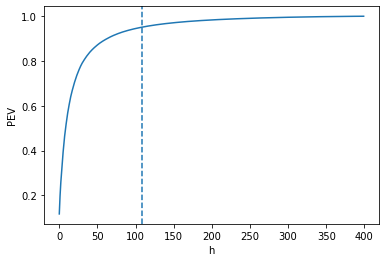
\includegraphics[width=\linewidth]{h0pca.png}
\caption{All Standardized Data} \label{fig:a}
\end{subfigure}\hspace*{\fill}
\begin{subfigure}{0.4\textwidth}
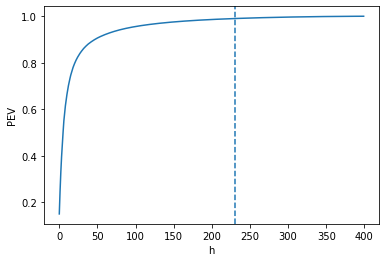
\includegraphics[width=\linewidth]{hbit.png}
\caption{Bitstream} \label{fig:b}
\end{subfigure}

\medskip
\begin{subfigure}{0.4\textwidth}
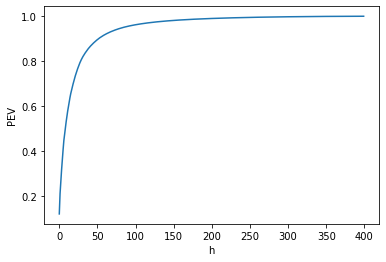
\includegraphics[width=\linewidth]{hcon.png}
\caption{Consolas} \label{fig:c}
\end{subfigure}\hspace*{\fill}
\begin{subfigure}{0.4\textwidth}
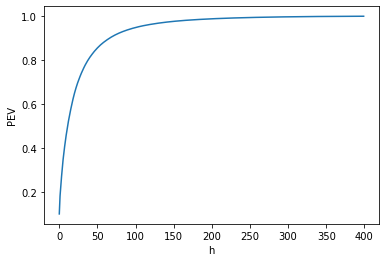
\includegraphics[width=\linewidth]{hebrim.png}
\caption{Ebrima} \label{fig:d}
\end{subfigure}
\caption{Principal Components for the Selection of H}
\label{h_pca}
\end{figure}

\question*{Training MLP$_0$ and MLP$^*$}
We next trained two different MLPs with hidden layers with our found h values. MLP$_0$ will have a hidden layer of size 108, while MLP$^*$ will have a hidden layer of size 643.\\\\
The training of MLP$_0$ was relatively straightforward. We selected the ADAM optimizer with cross-entropy as the loss function. We utilized tensorflow to learn the MLP's weights and biases, of which there are 404h+3. Therefore, MLP$_0$ learned 43,635 parameters. We set the batch size of the learning equal to the square root of the size of the training set, giving us a batch size of 71. The learning took approximately 40 seconds computing time in Google Colab.\\\\
The decrease in loss on both the training and testing sets is displayed in Figure \ref{MLP0}. The loss of the testing set begins to stabilize around epoch 50 and settled at about 0.2.  The loss of the training set at epoch 50 was approximately 0.05.
Overfit begins around epoch 80, as this is when the loss on the testing set begins to increase, and the loss on the training set reaches 0. The learning should stop at the minimum of these two values, which for us was epoch 50.\\

\begin{figure}[H]
    \centering
    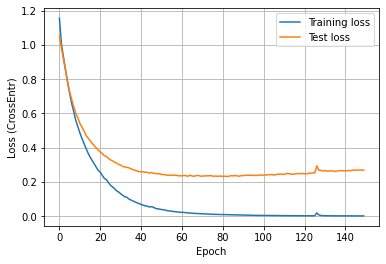
\includegraphics[width=10cm]{mlp0_learning.png}
    \caption{Performance of MLP$_0$}
    \label{MLP0}
\end{figure}

Since MLP$^*$'s h is large, we decided to apply sparsity learning to restrict the number of active neurons in the hidden layer. If MLP$^*$ learned every weight and threshold for all of its neurons, it would have to learn 259,775 parameters. Instead, sparsity learning allows MLP$^*$ to learn far fewer parameters than full learning. \\\\
We used values of 10\% and 20\% sparsity for MLP$^*$. Training each network took about thirty seconds each computing time in Google Colab. The performance on the training and testing sets for each is displayed in Figure \ref{MLP*}. Since it had access to more neurons, MLP$^*$ learned faster than MLP$_0$ at both sparsity levels, stabilizing at about the 20th epoch. However, its loss on both the training and testing sets was higher than MLP$_0$'s, as the cross-entropy of the testing set never reached 0.2, Instead hovering around 0.3. However, there is no obvious sign of overfit as the loss on the testing set never really increases, apart from random spikes. Nevertheless, learning at both sparsity levels should stop at the stabilization time, which was the 20th epoch.

\begin{figure}[h]
\begin{subfigure}{0.5\textwidth}
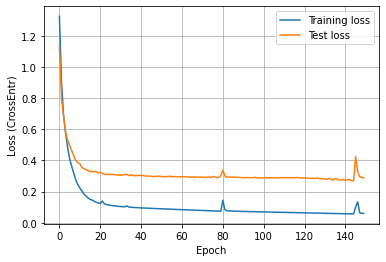
\includegraphics[width=\linewidth]{mlp_10.png}
\caption{MLP$^*$ at Sparsity Level = 10\%} \label{fig:a}
\end{subfigure}\hspace*{\fill}
\begin{subfigure}{0.5\textwidth}
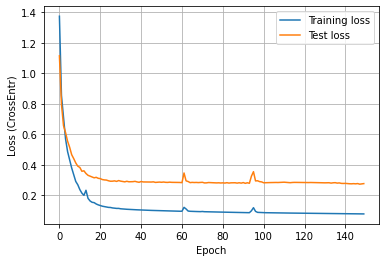
\includegraphics[width=\linewidth]{mlp_20.png}
\caption{MLP$^*$ at Sparsity Level = 20\%} \label{fig:b}
\end{subfigure}
\caption{Performance of MLP$^*$ at Two Sparsity Levels}
\label{MLP*}
\end{figure}

\question*{Confusion Matrices of MLP$_0$ and MLP$^*$}
Confusion matrices for MLP$_0$ at the 50th epoch are displayed in Table \ref{conf_MLP0}. True classes are along the columns, and predicted classes are across the rows. The classifier was completely accurate on the training set, and it performed reasonably well on the testing set with a global accuracy of 90.3\%. Most of the confusion is between fonts Consolas and Ebrima; every classifier we have tried previously - random forest, support vector machines, etc. - likewise had trouble distinguishing between these two fonts. MLP$_0$ performed on the same level as our previous best random forest, so the technique is promising at this early stage.\\\\
Confusion matrices for MLP$^*$ stopping at the 20th epoch are provided in Table \ref{conf_MLP*10} and Table \ref{conf_MLP*20}. Both MLP$^*$s performed well on the training set, with close to 100\% accuracy, while their performance on the testing sets was both around 92\%, with 20\% sparsity being slightly more accurate. Once again the difficulty lay in differentiating between Consolas and Ebrima, though  both MLP$^*$s were slightly better at this than MLP$_0$.

\begin{table}[H]
    \centering
    \subfloat[Training Set]{\begin{tabular}{c|ccc}
         &BITSTREAM&CONSOLAS&EBRIMA\\\hline
         BITSTREAM&1.000&0.000&0.000\\
         CONSOLAS&0.000&1.000&0.000\\
         EBRIMA&0.000&0.000&1.000\\\hline
         Global Accuracy&1.000
    \end{tabular}}\\
    \subfloat[Testing Set]{\begin{tabular}{c|ccc}
         &BITSTREAM&CONSOLAS&EBRIMA\\\hline
         BITSTREAM&0.991&0.004&0.007\\
         CONSOLAS&0.004&0.857&0.147\\
         EBRIMA&0.004&0.139&0.846\\\hline
         Global Accuracy&0.903&95\% CI: (0.887, 0.919)
    \end{tabular}}
    \caption{Confusion Matrices for MLP$_0$ at the 50th Epoch}
    \label{conf_MLP0}
\end{table}

\begin{table}[H]
    \centering
    \subfloat[Training Set]{\begin{tabular}{c|ccc}
         &BITSTREAM&CONSOLAS&EBRIMA\\\hline
         BITSTREAM&1.000&0.000&0.000\\
         CONSOLAS&0.000&1.000&0.001\\
         EBRIMA&0.000&0.000&0.999\\\hline
         Global Accuracy&0.999
    \end{tabular}}\\
    \subfloat[Testing Set]{\begin{tabular}{c|ccc}
         &BITSTREAM&CONSOLAS&EBRIMA\\\hline
         BITSTREAM&0.998&0.000&0.006\\
         CONSOLAS&0.002&0.876&0.142\\
         EBRIMA&0.000&0.124&0.852\\\hline
         Global Accuracy&0.914&95\% CI: (0.899, 0.929)
    \end{tabular}}
    \caption{Confusion Matrices for MLP$^*$ (Sparsity = 10\%) at the 20th Epoch}
    \label{conf_MLP*10}
\end{table}

\begin{table}[H]
    \centering
    \subfloat[Training Set]{\begin{tabular}{c|ccc}
         &BITSTREAM&CONSOLAS&EBRIMA\\\hline
         BITSTREAM&1.000&0.000&0.000\\
         CONSOLAS&0.000&1.000&0.000\\
         EBRIMA&0.000&0.000&1.000\\\hline
         Global Accuracy&1.000
    \end{tabular}}\\
    \subfloat[Testing Set]{\begin{tabular}{c|ccc}
         &BITSTREAM&CONSOLAS&EBRIMA\\\hline
         BITSTREAM&0.996&0.002&0.006\\
         CONSOLAS&0.002&0.884&0.119\\
         EBRIMA&0.002&0.114&0.875\\\hline
         Global Accuracy&0.922&95\% CI: (0.907, 0.937)
    \end{tabular}}
    \caption{Confusion Matrices for MLP$^*$ (Sparsity = 20\%) at the 20th Epoch}
    \label{conf_MLP*20}
\end{table}

\question*{Choosing the Best MLP$^*$}
From Tables \ref{conf_MLP*10} and \ref{conf_MLP*20}, we can see that the MLP$^*$ at 20\% sparsity is slightly better than the MLP$^*$ at 10\% sparsity, with a one percentage point greater  point estimate of global accuracy. However, the 95\% confidence intervals show some overlap such that the MLPs appear to perform similarly. Since the network with 20\% sparsity is slightly higher, though, we will say it is the best. Hence, the notation MLP$^*$ will refer exclusively to the network trained at 20\% sparsity.

\question*{Average Activity of MLP$^*$'s Neurons}
It is instructive to examine the average activity of MLP$^*$'s neurons. Average activity refers to how often a given neuron is used (and hence is updated by the MLP) when processing cases for classification. If the neurons show high levels of activity then the MLP is using the majority of its neurons for the majority of the cases, which implies the MLP is efficient. If the accuracy is also good, this suggests that the chosen size of h is likely the most robust to new cases.\\\\
Figure \ref{neurons} shows the histogram for MLP$^*$'s neurons' average activity. The distribution is approximately normal and it is centered at a mean of 0.469 with a standard deviation of 0.037. On average, the neurons are used by the MLP$^*$ relatively equally.

\begin{figure}[H]
    \centering
    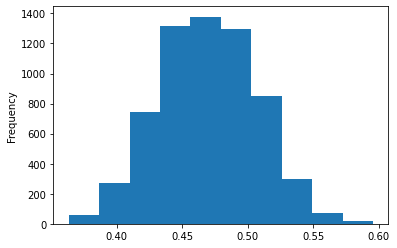
\includegraphics[width=10cm]{mlp20_neurons.png}
    \caption{Average Activity of Neurons on MLP$^*$}
    \label{neurons}
\end{figure}

\question*{Empirical Sparsity of MLP$^*$}
%***PLEASE CHECK THIS PART ESPECIALLY***
The most inactive neuron had an average activity of 0.374 while the most active neuron had an average activity of 0.610. No neurons meet the empirical sparsity level of less than half the average activity. All the neurons updated their states quite frequently when they were allowed to do so.

\question*{Principal Components of the Hidden Layer}
We proceeded to train an autoencoder based off the weights and biases learned by MLP$^*$ at its stopping time of the 20th epoch. First we compute the number of principal components required to explain 95\% of MLP$^*$'s hidden layer Z. This is displayed in Figure \ref{z_pca}. \textbf{191 principal components} were required to explain 95\% of the variance across Z. 

\begin{figure}[H]
    \centering
    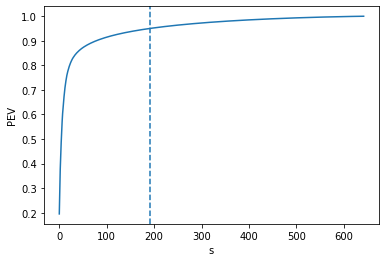
\includegraphics[width=10cm]{zpca.png}
    \caption{PCA on the Hidden Layer, Z}
    \label{z_pca}
\end{figure}

\question*{Autoencoding of Z}
Encoding of Z may lead to an improvement in the performance of the classifier. A good compression of Z, Z*, could be easier for a neural network to learn and classify than the original features were.\\\\
We set the number of principal components required to explain Z, 191, as the dimension of our autoencoder's hidden layer. We trained an MLP comprised of the following dimensions: 643 for the input vector Z; 191 for the hidden layer; and 643 for the output layer. Recall that the our dimension of 643 for Z is equivalent to the size of MLP$^*$'s hidden layer. The loss function of our autoencoder was the Mean Squared Error (MSE).\\\\
Performance of this encoding is displayed in Figure \ref{zperf}. The MSE of the autoencoding stabilized at approximately 0.006. The ratio of root(MSE) to the average length of Z, known as the normalized error, was 0.164. This implies that the compression of Z, Z*, misses the true value of Z by about 0.164, on average. A desired threshold for this type of autoencoding is a normalized error of less than 0.1. Thus so the encoding may not be very useful for our purpose.

\begin{figure}
    \centering
    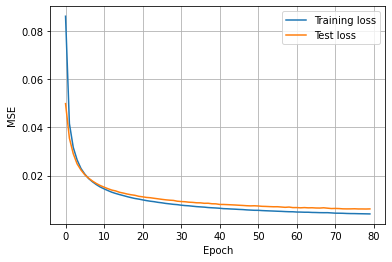
\includegraphics[width=10cm]{zperf.png}
    \caption{Performance of Autoencoding the Hidden Layer}
    \label{zperf}
\end{figure}

\question*{Training a Short MLP with the Encoding}
The weights learned from Z*, were next used to classify the fonts. There is no hidden layer in this MLP, just the weights and biases going from Z* to the three-dimensional output layer. This is then passed through the softmax activation function (this last step being a deterministic process). as this is a classification problem, we returned to using cross-entropy as our loss function. The results are displayed in the following section.

\question*{Deploying the Two-Layer MLP}
We then concatenated the layers together. The flow of the MLP is as follows: the standardized input data (dimension of 400), MLP$^*$'s hidden layer (dimension of 643), the encoding of this hidden layer (dimension of 191), and the output layer (dimension of 3).\\\\
The performance of this long MLP, MLP**, is as in Figure \ref{long_mlp}, with confusion matrices in Table \ref{conf_MLP**}. The loss stabilized near 0.3 at about the 20th epoch. Hence, the performance of MLP** appears similar to the performance of MLP*. Table \ref{conf_MLP**} provides confirmation, as the 95\% confidence interval of its global accuracy contains similar values to MLP*.\\\\
In fact, all the MLPs this paper considers - MLP$_0$, MLP$^*$, and MLP** - have similar performances on the font classification problem. Increasing the size of the hidden layer did not increase performance and the introduction of an autoencoder to the hidden layer also did not increase performance. Since this is image data, a Convolution Neural Network may be appropriate to implement, but that is beyond the scope of this homework.

\begin{figure}[H]
    \centering
    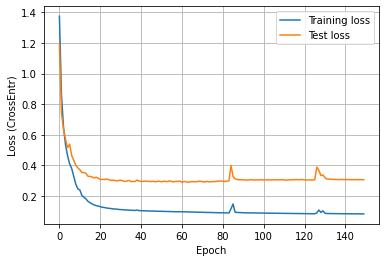
\includegraphics[width=10cm]{mlp_aec.png}
    \caption{Performance of MLP**}
    \label{long_mlp}
\end{figure}

\begin{table}[H]
    \centering
    \subfloat[Training Set]{\begin{tabular}{c|ccc}
         &BITSTREAM&CONSOLAS&EBRIMA\\\hline
         BITSTREAM&1.000&0.000&0.000\\
         CONSOLAS&0.000&1.000&0.000\\
         EBRIMA&0.000&0.000&1.000\\\hline
         Global Accuracy&1.000
    \end{tabular}}\\
    \subfloat[Testing Set]{\begin{tabular}{c|ccc}
         &BITSTREAM&CONSOLAS&EBRIMA\\\hline
         BITSTREAM&0.981&0.000&0.007\\
         CONSOLAS&0.006&0.863&0.111\\
         EBRIMA&0.013&0.137&0.882\\\hline
         Global Accuracy&0.911&95\% CI: (0.895, 0.927)
    \end{tabular}}
    \caption{Confusion Matrices for MLP**}
    \label{conf_MLP**}
\end{table}

\newpage
\lstinputlisting{code.py}
\end{document}
